\iffalse
\documentclass[journal,12pt,twocolumn]{IEEEtran}
\usepackage{amsmath,amssymb,amsfonts,amsthm}
\usepackage{txfonts}
\usepackage{tkz-euclide}
\usepackage{listings}
\usepackage{gvv}
\usepackage[latin1]{inputenc}
\usepackage{adjustbox}
\usepackage{array}
\usepackage{tabularx}
\usepackage{pgf}
\usepackage{lmodern}
\usepackage{circuitikz}
\usepackage{tikz}
\usepackage{graphicx}

\begin{document}
\bibliographystyle{IEEEtran}

\vspace{3cm}

\title{}
\author{EE23BTECH11054 -  Sai Krishna Shanigarapu$^{*}$
}
\maketitle
\newpage
\bigskip

% \renewcommand{\thefigure}{\theenumi}
% \renewcommand{\thetable}{\theenumi}

\section*{Gate EE 2023}
54. \hspace{2pt}The circuit shown in the figure is initially in the steady state with the switch K in open condition and $\overline{K}$ in closed condition. The switch K is closed and $\overline{K}$ is opened simultaneously at the instant $t = t_1$, where $t_1 > 0$. The minimum value of $t_1$ in milliseconds such that there is no transient in the voltage across the 100 $\mu F$ capacitor, is \rule{1cm}{0.15mm} (Round off to 2 decimal places).\\ 
\hfill(GATE EE 2023)

\begin{figure}[ht]
  \centering
  \begin{adjustbox}{width=\columnwidth}
      \begin{circuitikz}[american]
   \draw (0,0) to [isource, l=1A] (0,4) ;
   \draw (0,0) to [short] (3,0) to [C = 0.01F] (3,4) to [short] (6,4) to [R = 100 $\Omega$] (6,2) to [L = 1H] (6,0) to [short] (9,0) to [R = 25 $\Omega$] (9,4) to [short] (6,4) ;
   \draw (3,0) to [short] (6,0) ;
   \draw (0,4) to [ospst = $S_1$] ++(3,0); 
   \draw (7.5,4) to [cspst = $S_2$] ++(0,-2);
   \draw (7.5,2) to [short] (6,2) ;
   \draw (3,4) to [short ,i = $i_c$] (3,3);
   
\end{circuitikz}

  \end{adjustbox}
  \caption{Circuit 1}
\end{figure}

\solution
\fi
\begin{enumerate}
\item Switch K is open and $\overline{K}$ is closed.
\begin{figure}[ht]
  \centering
          \begin{circuitikz}[american]
        \draw (0,7) to [R=10$\Omega$] (0,2) to [short] (3,2) to [isource, l=$1\angle{0^\circ}$] (3,7) to [short] (0,7);
        \draw (3,7) to [short, i=$I_1$] (7,7);
        \draw (3,2) to [short] (7,2);
        \draw (7,7) -- ++(0,-1.5)
        to [open, v=$V_1$, o-o] ++(0,-1.5) -- ++(0,-2);
\end{circuitikz}


  \caption{K is open and $\overline{K}$ is closed}
\end{figure}

Using Current divider rule,
\begin{align}
   I_1\brak{j\omega} &= \frac{10}{10+\frac{1}{j\omega C}}\\
   V_1\brak{j\omega} &= \frac{10}{1+10j\omega C}\\
   \abs{V_1\brak{j\omega}} &= 5\sqrt{2}
 \end{align}
 From Table \ref{tab:Gate.ee.54.1}
 \begin{align}
   V_1\brak{t} &= 5\sqrt{2}\sin\brak{\omega t - \frac{\pi}{4}} \label{eq:1.gate.ee.23.54}
\end{align}


\item Switch K is closed and $\overline{K}$ is open.

\begin{figure}[ht]
  \centering
      %\begin{circuitikz}[american]
        %\draw (0,0) to [R=10$\Omega$] (1.5,0) to [battery2=5V] (4,0);
        %\draw (0,0) to [short] (0,3) to [short] (4,3) to [C=100$\mu$F, %v=$V_c\brak{\infty}$] (4,0) ;
%\end{circuitikz}

\begin{circuitikz}[american]
    \draw (0,0) to [R=10$\Omega$] (1.5,0) to [battery2=$\frac{5}{s}$] (4,0);
    \draw[<-, thick] (1.5,1) arc (-90:90:0.5) node[midway, left] {$I(s)$};
    \draw (0,0) to [short] (0,3) to [short] (4,3) to [C=$\frac{10^4}{s}$, v=$V_c\brak{s}$] (4,0);
\end{circuitikz}


  \caption{K is closed and $\overline{K}$ is open}
\end{figure}


The capacitor is charged. Thus, acts as a voltage source.\\
From eq\brak{\ref{eq:1.gate.ee.23.54}} and Table \ref{tab:Gate.ee.54.2}
\begin{align}
    V_1\brak{s} &= \frac{5000 - 5s}{s^2 + 10^6} \\
    I\brak{s} &= \frac{\frac{5}{s} - V_1\brak{s}}{10 + \frac{10^4}{s}}\\
    V_c\brak{s} &= \frac{5}{s} - 10\brak{\frac{5-V_1\brak{s}}{1+10^{-3}s}}
\end{align}
\end{enumerate}

For transient analysis,
\begin{align}
    \frac{5-V_1\brak{s}}{1+10^{-3}s} &= 0\\
    \implies V_1\brak{s} &= 5\\
    \frac{10^7}{\brak{s^2+10^6}\brak{s+10^3}} &= \frac{5}{s}\\
    \frac{5}{s+10^3} + \frac{10^3-s}{s^2 + 10^6} &= \frac{5}{s}\\
    \frac{-s}{s^2+10^6} + \frac{10^3}{s^2 + 10^6} + \frac{1}{s+10^3} &= \frac{1}{s}
\end{align}
From Table \ref{tab:Gate.ee.54.2}
\begin{align}
    -\cos\brak{1000t_1}+\sin\brak{1000t_1}+e^{-10^3 t_1} &= 1\\
    \implies t_1 \approx 1.57\text{msec}
\end{align}

\begin{table}[ht]
       \setlength{\arrayrulewidth}{0.3mm}
\setlength{\tabcolsep}{20pt}
\renewcommand{\arraystretch}{1.3}



\begin{tabular}{|c|c|c|}
\hline

Parameter& Description & Remarks\\
\hline
$\omega$ & frequency of sine-wave & 1000 rad s$^{-1}$\\
\hline
$V_1\brak{t}$ & Voltage across capacitor & $\abs{V_1\brak{j\omega}}\sin\brak{\omega t - \angle{V_1\brak{j\omega}}}$\\
\hline
$\angle{V_1\brak{j\omega}} $ & phase of $V_1\brak{j\omega}$ & $\frac{-\pi}{4}$\\
\hline
$C$ & Capacitance & 100$\mu$F\\
\hline

\end{tabular}






    \caption{Parameters}
    \label{tab:Gate.ee.54.1}

\end{table}


\begin{table}[ht]
    \setlength{\arrayrulewidth}{0.3mm}
\setlength{\tabcolsep}{20pt}
\renewcommand{\arraystretch}{1.3}


\begin{tabular}{|c|c|}
\hline

S Domain & Time Domain\\
\hline
$\frac{1}{s}$ & $u\brak{t}$\\
\hline
$\frac{-s}{a^2+s^2}$ & $-\cos\brak{at}$\\
\hline
$\frac{a}{a^2+s^2}$ & $\sin\brak{at}$\\
\hline
$\frac{1}{s+a}$ & $e^{-at}$\\
\hline

\end{tabular}





    \caption{Laplace transforms}
    \label{tab:Gate.ee.54.2}
\end{table}

\begin{figure}[htbp]
    \centering
    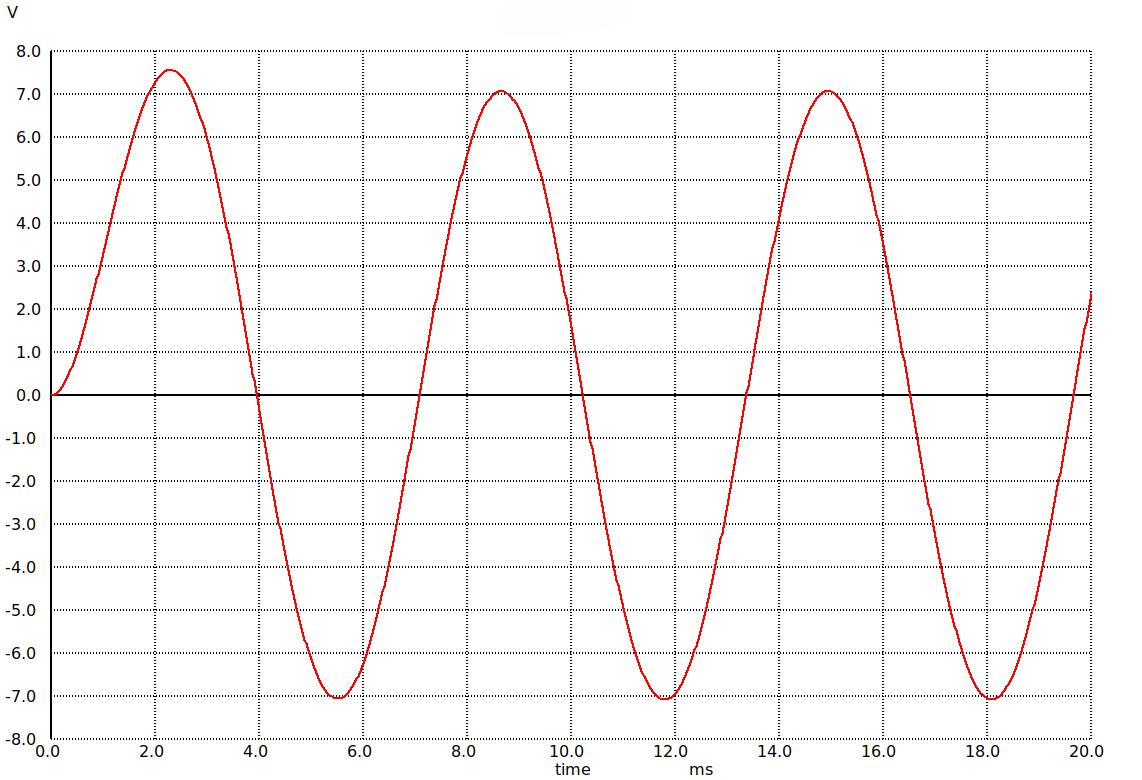
\includegraphics[width=1\columnwidth]{2023/EE/54/figs/fig1.png}
    \caption{plot of $V_1$ vs time}
\end{figure}

\begin{figure}[htbp]
    \centering
    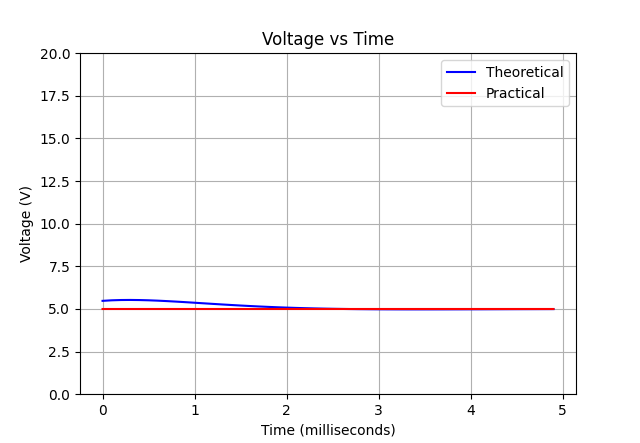
\includegraphics[width=1\columnwidth]{2023/EE/54/figs/fig3.png}
    \caption{plot of $V_c$ vs time}
\end{figure}

%\end{document}
